\chapter{Classification} \label{chap:chap-3}


% add citation for the chapter if it is a reprint


% remove the following and add your chapter text
\section{Introduction}
A classifier was trained to predict what metals and ligands were used to generate each voltammogram to demonstrate further the feasibility of using this encoding technique for various machine learning tasks. It is important to note that the dataset used is relatively small for a deep learning task. For training, the dataset was split with 80\% for training, 10\% for validation, and 10\% for testing. 5-fold cross-validation, a technique for assessing the performance of a machine learning model by dividing the dataset into k subsets, training the model on k-1 subsets, and evaluating it on the remaining subset for each subset, is also used \cite{hastie_09_elements-of.statistical-learning}. An important insight to consider is the similarity between voltammetry data and images. After all, each point has a potential and current value, similar to an image\textquotesingle s RGB values. The main difference is that an image is 2-dimensional while voltammetry data is 1-dimensional. Many previous works have used convolutional neural networks (CNNs) for classification tasks \cite{SHARMA2018377}. Using this as inspiration, the proposed model architecture for voltammetry data classification uses 1-dimensional convolutional layers. 
\section{Variational Autoencoders}
\begin{figure}[h!]
  \centering
    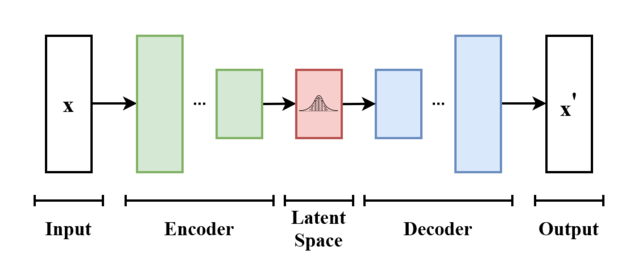
\includegraphics[width=1.0\textwidth]{figures/autoencoder_architecture.png}
    \caption{Autoencoder Diagram}
    \label{autoencoder_diagram}
    Input is encoded into latent space and then recreated using decoder
\end{figure}
Since one major challenge is the dataset size, one method to address this is to create synthetic data. 
A variational autoencoder (VAE) is similar to the autoencoder neural network architecture shown in Figure \ref{autoencoder_diagram}, with the main difference being that VAEs connects the encoder to its decoder through a probabilistic latent space that corresponds to the parameters of a variational distribution \cite{PinheiroCinelli2021}. The encoder maps each point from the dataset into a distribution within the latent space rather than a single point in that space. The distribution is typically Gaussian with a mean and a variance. Once the VAE is trained, different points can be sampled from the learned latent space distribution. These samples represent different configurations of the input data in the latent space. The sampled points from the latent space are fed into the decoder network, which reconstructs the input data corresponding to those points and generates a diverse set of synthetic data samples that resemble the original data distribution. The variability in the latent space allows for the generation of novel and diverse data samples that capture the underlying characteristics of the training data.
\section{Conditional Variational Autoencoders}
While traditional VAEs learn a latent space for the dataset, conditional variational autoencoders (CVAEs) expand this concept by introducing conditional dependencies between the input data and the latent variables. In the context of generating synthetic data, CVAEs offer a more controlled approach by allowing the generation process to be conditioned on additional information, such as class labels or other attributes associated with the data.
By conditioning the generation process on known attributes or labels, CVAEs can generate synthetic data samples that capture the underlying data distribution and adhere to specific conditions or constraints defined by the conditioning variables. This enables the targeted generation of synthetic data for different classes or categories when labelled data is lacking. In this case, the metal and ligand are encoded using one-hot encoding and passed to the decoder to generate data from the same class. 
\section{Classifier Model Architecture}
\begin{figure}[!h]
  \centering
    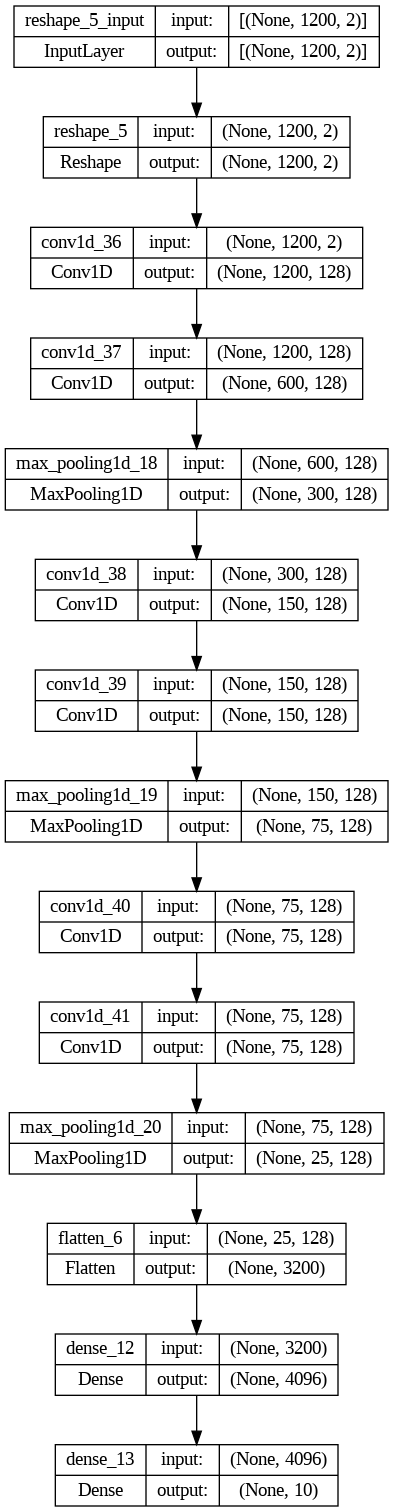
\includegraphics[width=0.25\textwidth]{figures/model_architecture.png}
    \caption{Classification Model Architecture}
    \label{model_arch}
\end{figure}
The classifier architecture can be seen in Figure \ref{model_arch}. The model consists of several convolutional and max-pooling layers to encode the data and reduce dimensions. All layers except for the output layer use the ReLU activation function. The output layer is a dense layer with ten units, one for each metal/ligand, and a softmax activation function. The Adam optimizer and categorical cross-entropy loss are used to train the model. Additionally, the model uses L2 regularization and early stopping to prevent overfitting and ensure smooth convergence. The Glorot uniform initializer is used for weight initialization to facilitate better gradient flow and prevent exploding gradients. 
\section{Results and Discussion}
\begin{table}[!h]
\begin{center}
\begin{tabular}{c|c|c|c|c|c|c}
Model & Fold 1 Acc & Fold 2 Acc & Fold 3 Acc & Fold 4 Acc & Fold 5 Acc & Avg Acc\\
\hline
CV Ligands & 75.13\% & 80.29\% & 69.65\% & 76.40\% & 78.82\% & 76.06\%\\
CV Metals & 79.24\% & 82.50\% & 81.36\% & 80.11\% & 78.97\% & 80.44\%\\
DPV Ligands & 30.00\% & 35.00\% & 25.00\% & 25.00\% & 30.00\% & 29.00\%\\
DPV Metals & 25.00\ & 30.00\% & 25.00\% & 20.00\% & 25.00\% & 25.00\%\\
\end{tabular}
\caption{Classification Accuracy}
\label{classification_results}
\end{center}
\end{table}
Separate classifiers were trained, each with a unique task of classifying CV ligands, CV metals, DPV ligands, and DPV metals. 
The accuracy of the classifiers can be seen in Table \ref{classification_results}, and the results were much better for the CV data than the DPV data. This difference can likely be attributed to the size of the datasets. 
\begin{table}[!h]
\begin{center}
\begin{tabular}{c|c|c|c|c|c|c}
Model & Fold 1 Acc & Fold 2 Acc & Fold 3 Acc & Fold 4 Acc & Fold 5 Acc & Avg Acc \\
\hline
CV Ligands & 77.86\% & 78.50\% & 80.94\% & 72.01\% & 73.02\% & 76.47\%\\
CV Metals & 85.00\% & 81.23\% & 84.19\% & 83.10\% & 78.75\% & 82.45\%\\
DPV Ligands & 25.00\% & 25.00\% & 15.00\% & 20.00\% & 20.00\% & 21.00\%\\
DPV Metals & 25.00\% & 20.00\% & 20.00\% & 25.00\% & 25.00\% & 23.00\%
\end{tabular}
\caption{Classification Accuracy with Synthetic Data}
\label{vae_classification_results}
\end{center}
\end{table}
After incorporating synthetic data generated with the CVAE into the training process, accuracy significantly improved for classifying CV data, as seen in Table \ref{vae_classification_results}. However, the DPV ligands classifier saw a decrease in performance. Again, this is likely due to the size of the dataset. Several key considerations impact the quality of data generated by VAEs, especially when dealing with small datasets. Firstly, the quality and diversity of the original data influence the effectiveness of the synthetic data produced by VAEs. With limited variation or complexity in a small dataset, the VAE might struggle to accurately capture the proper underlying data distribution, potentially resulting in synthetic data that fails to represent the characteristics of the actual data fully. This mismatch can detrimentally affect classifier performance. 

Additionally, the risk of overfitting is heightened in small datasets, where the classifier may excessively specialize in training data patterns that do not generalize well. Introducing synthetic data from a VAE can compound this issue if the VAE itself overfits the small dataset, producing synthetic data overly similar to the training data, which provides minimal additional information for the classifier and can lead to decreased performance on unseen data. VAEs implicitly learn the probability distribution of the input data. However, suppose the actual data distribution is significantly different from the distribution learned by the VAE due to the small dataset size. In that case, the synthetic data generated by the VAE may not accurately represent the true data distribution. This distribution mismatch can confuse the classifier, as it may encounter data points in the synthetic dataset that deviate from the real data distribution, leading to suboptimal performance.
\begin{table}[!h]
\begin{center}
\begin{tabular}{c|c|c|c|c}
 & Precision & Recall & F1-Score & Support\\
\hline
Metal 1 & 0.88 & 0.88 & 0.88 & 8\\
Metal 2 & 0.80 & 1.00 & 0.89 & 8\\
Metal 3 & 1.00 & 1.00 & 1.00 & 4\\
Metal 4 & 1.00 & 0.83 & 0.91 & 12\\
Metal 5 & 1.00 & 0.71 & 0.83 & 7\\
Metal 6 & 0.88 & 0.78 & 0.82 & 9\\
Metal 7 & 0.82 & 0.90 & 0.86 & 10\\
Metal 8 & 0.50 & 0.40 & 0.44 & 5\\
Metal 9 & 0.78 & 1.00 & 0.88 & 7\\
Metal 10 & 0.82 & 0.90 & 0.86 & 10\\
\hline
Accuracy & & & 0.85 & 80\\
Macro Avg & 0.85 & 0.84 & 0.84 & 80\\
Weighted Avg & 0.86 & 0.85 & 0.85 & 80
\end{tabular}
\caption{CV Metals Classification Report}
\label{cv_metal_report}
\end{center}
\end{table}
Table \ref{cv_metal_report} provides insights into the precision, recall, and F1-score when classifying each metal type, along with the number of instances (support) for each metal type. Precision indicates the proportion of true positive predictions among all positive predictions, while recall measures the proportion of true positives that were correctly identified. F1-score, the harmonic mean of precision and recall, provides a balanced measure between the two.
Overall, the classifier model achieved an accuracy of 85\%, indicating its effectiveness in classifying different metal types. However, it is important to note variations in performance across metal types. For instance, Metal 3 achieved perfect precision, recall, and F1-score, suggesting the model\textquotesingle s ability to  classify this particular metal type accurately. On the other hand, Metal 8 exhibited lower precision and recall scores, indicating potential challenges in distinguishing this metal type from others.
Both macro-average and weighted-average metrics hover around 0.85, indicating a reasonably balanced performance across all metal types. These metrics consider the average performance across all classes, with macro-average treating all classes equally, while weighted-average considers the contribution of each class based on its support.
\begin{table}[!h]
\begin{center}
\begin{tabular}{c|c|c|c|c}
 & Precision & Recall & F1-Score & Support\\
\hline
Ligand 1 & 0.88 & 0.78 & 0.82 & 9\\
Ligand 2 & 0.88 & 0.88 & 0.88 & 8\\
Ligand 3 & 0.75 & 0.86 & 0.80 & 7\\
Ligand 4 & 0.45 & 0.71 & 0.56 & 7\\
Ligand 5 & 0.78 & 0.70 & 0.74 & 10\\
Ligand 6 & 1.00 & 0.86 & 0.92 & 7\\
Ligand 7 & 0.71 & 0.50 & 0.59 & 10\\
Ligand 8 & 0.67 & 0.89 & 0.76 & 9\\
Ligand 9 & 1.00 & 0.67 & 0.80 & 3\\
Ligand 10 & 1.00 & 0.90 & 0.95 & 10\\
\hline
Accuracy & & & 0.78 & 80\\
MacroAvg & 0.81 & 0.77 & 0.78 & 80\\
WeightedAvg & 0.80 & 0.78 & 0.78 & 80
\end{tabular}
\caption{CV Ligands Classification Report}
\label{cv_ligands_report}
\end{center}
\end{table}
Table \ref{cv_metal_report} shows the classification report for classifying ligands. The classifier achieved an accuracy of 78\% overall, indicating its capability to classify different metal types to some extent. However, upon closer examination, there are notable variations in performance across metal types. For instance, Metal 6 demonstrates excellent precision, recall, and F1-score, suggesting the model\textquotesingle s proficiency in accurately classifying this metal type. Conversely, Metal 4 exhibits lower precision, recall, and F1-score, indicating challenges in distinguishing this metal type from others.
\begin{table}[!h]
\begin{center}
\begin{tabular}{c|c|c|c|c}
 & Precision & Recall & F1-Score & Support\\
\hline
Ligand 1 & 1.00 & 1.00 & 1.00 & 1\\
Ligand 2 & 0.00 & 0.00 & 0.00 & 2\\
Ligand 3 & 0.33 & 0.25 & 0.29 & 4\\
Ligand 4 & 0.33 & 0.33 & 0.33 & 3\\
Ligand 5 & 0.50 & 0.50 & 0.50 & 4\\
Ligand 6 & 0.00 & 0.00 & 0.00 & 1\\
Ligand 7 & 0.00 & 0.00 & 0.00 & 1\\
Ligand 8 & 0.00 & 0.00 & 0.00 & 0\\
Ligand 9 & 0.00 & 0.00 & 0.00 & 1\\
Ligand 10 & 1.00 & 0.33 & 0.50 & 3\\
\hline
Accuracy & & & 0.30 & 20\\
MacroAvg & 0.32 & 0.24 & 0.26 & 20\\
WeightedAvg & 0.42 & 0.30 & 0.33 & 20
\end{tabular}
\caption{DPV Ligands Classification Report}
\label{dpv_ligand_report}
\end{center}
\end{table}
\begin{table}[!h]
\begin{center}
\begin{tabular}{c|c|c|c|c}
 & Precision & Recall & F1-Score & Support\\
\hline
Ligand 1 & 0.33 & 1.00 & 0.50 & 2\\
Ligand 2 & 0.00 & 0.00 & 0.00 & 1\\
Ligand 3 & 0.25 & 0.50 & 0.33 & 2\\
Ligand 4 & 0.00 & 0.00 & 0.00 & 3\\
Ligand 5 & 0.00 & 0.00 & 0.00 & 1\\
Ligand 6 & 0.50 & 0.25 & 0.33 & 4\\
Ligand 7 & 0.00 & 0.00 & 0.00 & 2\\
Ligand 8 & 1.00 & 0.50 & 0.67 & 2\\
Ligand 9 & 0.00 & 0.00 & 0.00 & 3\\
Ligand 10 & 0.00 & 0.00 & 0.00 & 0\\
\hline
Accuracy & & & 0.30 & 20\\
MacroAvg & 0.23 & 0.25 & 0.20 & 20\\
WeightedAvg & 0.26 & 0.25 & 0.22 & 20
\end{tabular}
\caption{DPV Metals Classification Report}
\label{dpv_metal_report}
\end{center}
\end{table}
Table \ref{dpv_ligand_report} and Table \ref{dpv_metal_report} show the classification reports for DPV ligands and metals. However, the small sample size makes it difficult to draw definitive conclusions from this data. To further assess the performance of these classification models, receiving operating characteristic (ROC) curves and area under the ROC curve (AUC) values can be used to gain valuable insights into the discrimination capabilities and robustness of the models when distinguishing between various metals and ligands. ROC curves and AUC values help assess the robustness of the classification model by showing how well it performs across different thresholds and levels of noise. A smooth ROC curve with a high AUC suggests that the model can reliably discriminate between different metals and ligands even in the presence of noise or variability. 

Furthermore, there may be a need to choose a classification threshold that balances sensitivity and specificity according to specific requirements or constraints. ROC curves provide a visual aid for selecting an appropriate threshold based on the desired trade-off between true positives and false positives. For example, when integrating with an SDL, minimizing false positives (misclassification of metals or ligands) might be prioritized over maximizing true positives.
\begin{figure}[h!]
  \centering
    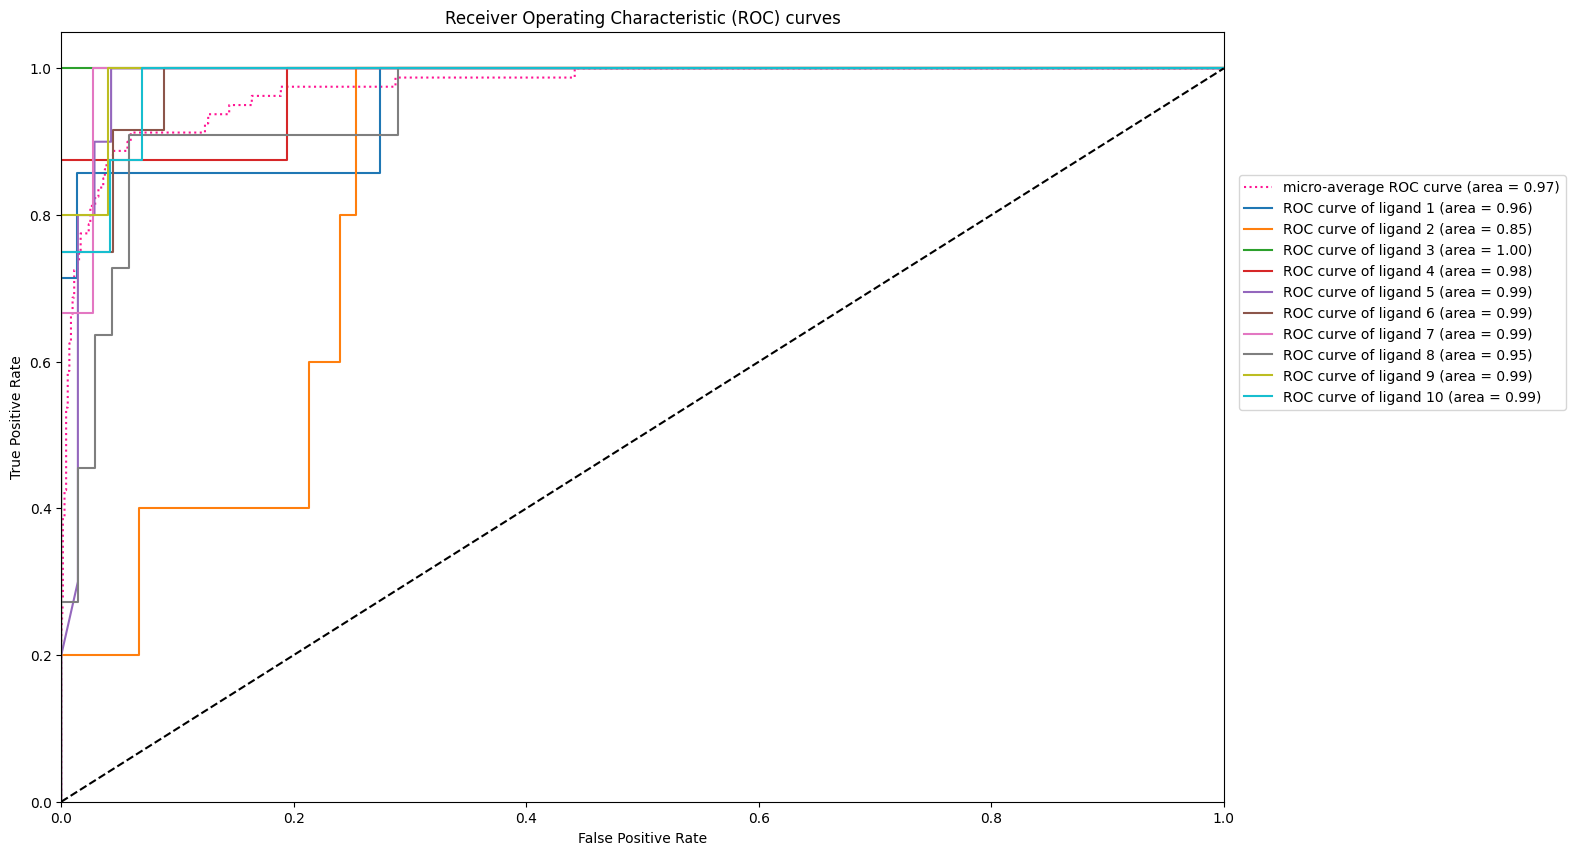
\includegraphics[width=1.0\textwidth]{figures/ligand_roc.png}
    \caption{CV Ligand ROC Curves}
    \label{ligand_roc}
\end{figure}
\begin{figure}[h!]
  \centering
    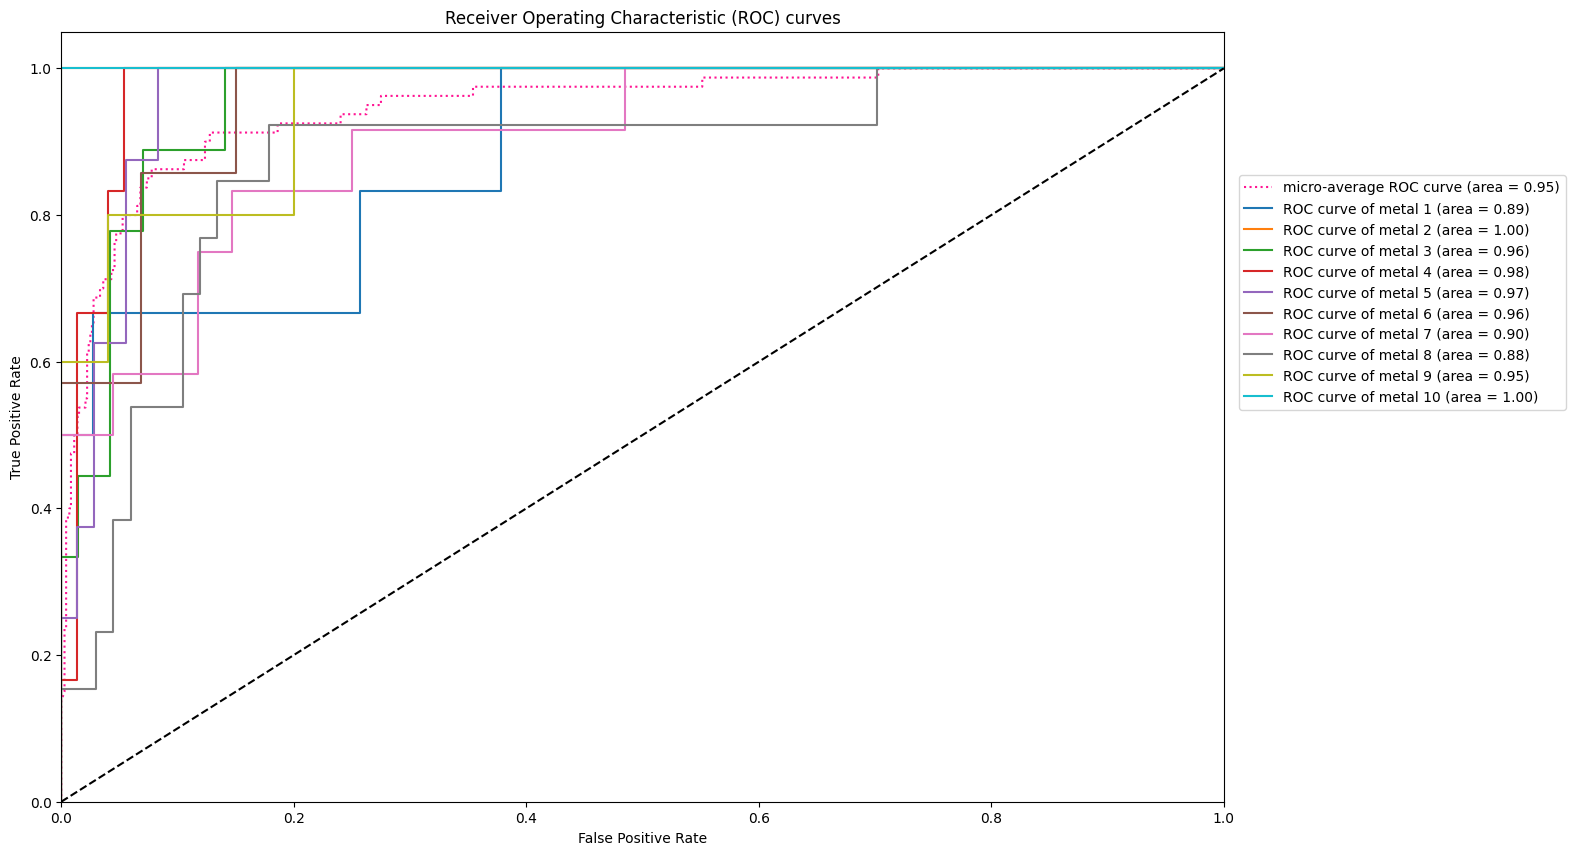
\includegraphics[width=1.0\textwidth]{figures/metal_roc.png}
    \caption{CV Metal ROC Curves}
    \label{metal_roc}
\end{figure}
The ROC curves in Figure \ref{ligand_roc} and Figure \ref{metal_roc} show good results for both metals and ligands. The area under the ROC curve (AUC) calculation summarized the ROC curve analysis into a scalar value, which ranges between 0 and 1. The closer the AUC score to value 1, the better the application’s overall performance.
\begin{figure}[h!]
  \centering
    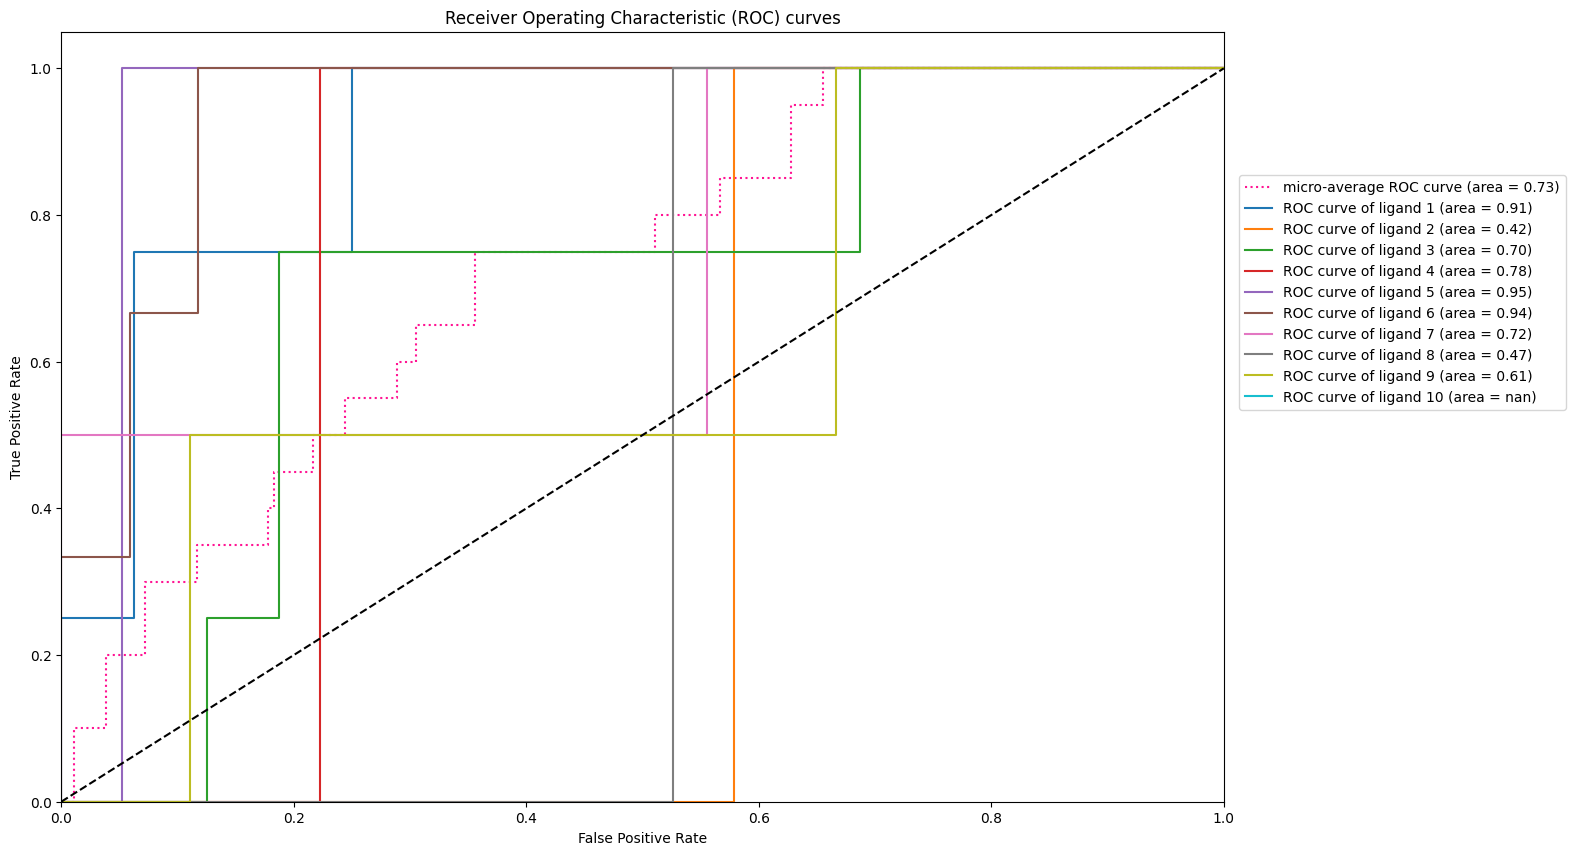
\includegraphics[width=1.0\textwidth]{figures/dpv_ligand_roc.png}
    \caption{DPV Ligand ROC Curves}
    \label{dpv_ligand_roc}
\end{figure}
\begin{figure}[h!]
  \centering
    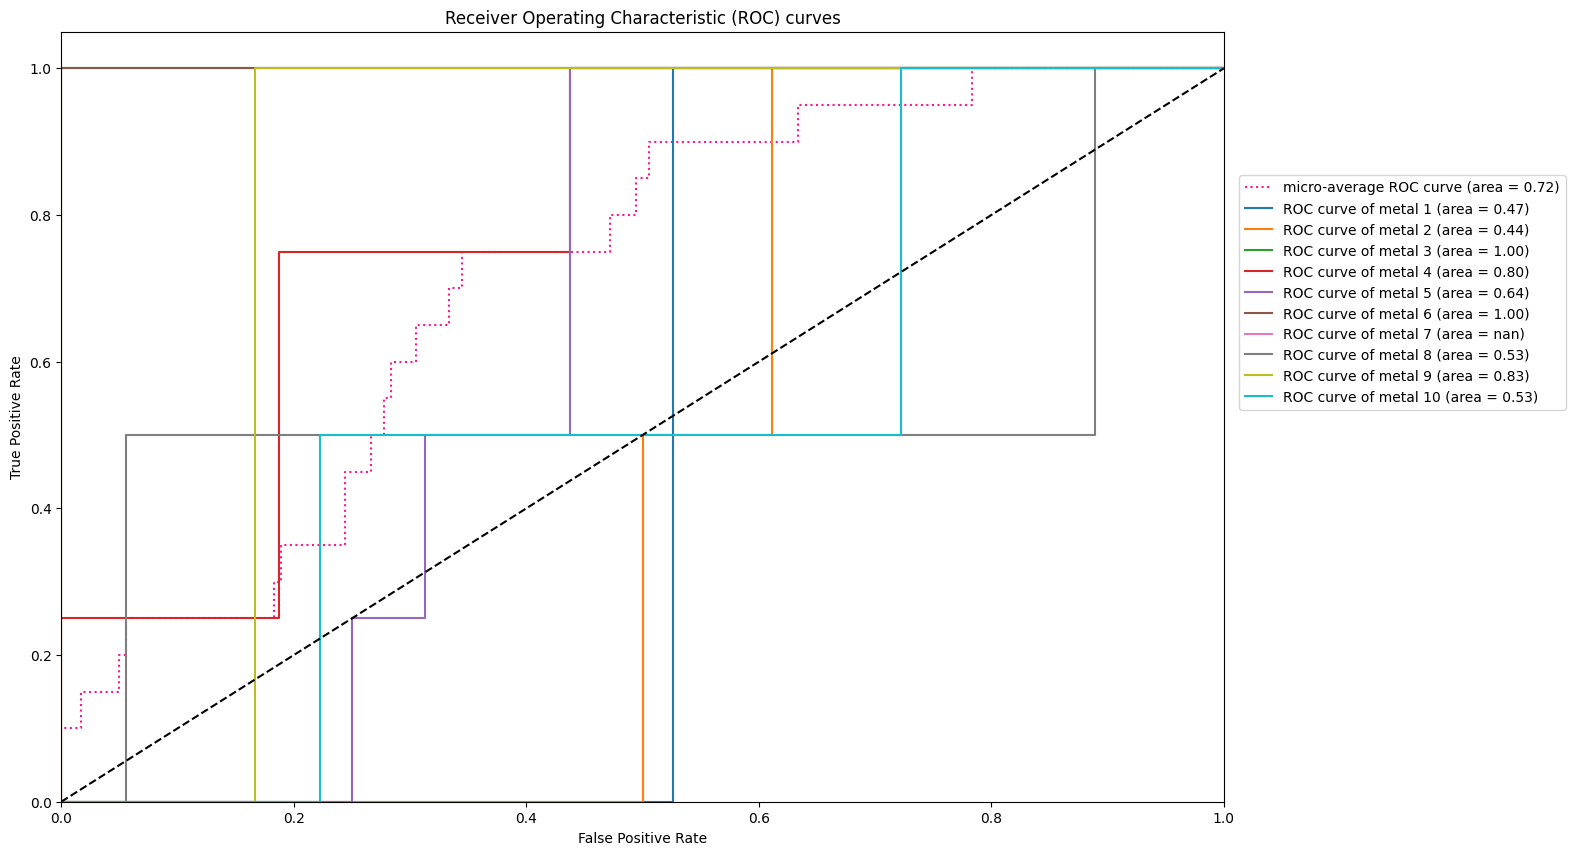
\includegraphics[width=1.0\textwidth]{figures/dpv_metal_roc.png}
    \caption{DPV Metal ROC Curves}
    \label{dpv_metal_roc}
\end{figure}
In Figure \ref{dpv_ligand_roc} and Figure \ref{dpv_metal_roc}, the ROC curves show that the classifier outperforms a random classifier by having an AUC value above 0.5. 
\begin{figure}[h!]
  \centering
    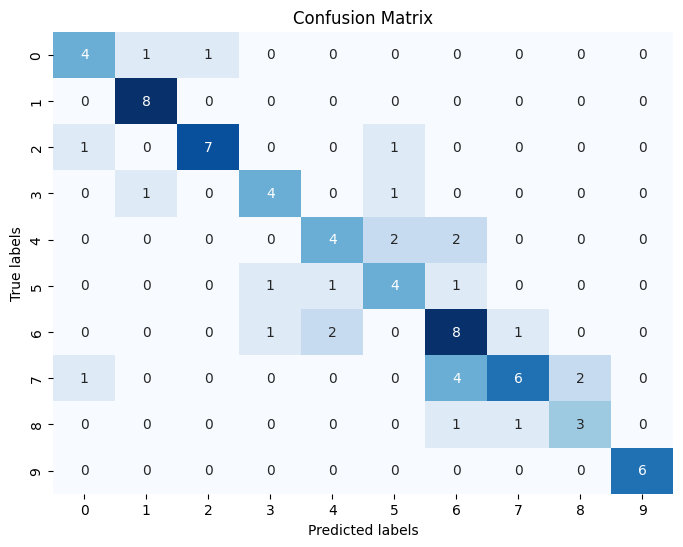
\includegraphics[width=1.0\textwidth]{figures/cv_ligand_matrix.png}
    \caption{CV Ligand Confusion Matrix}
    \label{cv_ligand_matrix}
\end{figure}
The data itself may cause issues with classification as some ligands and metals may be more difficult to distinguish than others. The confusion matrices are provided to investigate this.
From the confusion matrix for ligands \ref{cv_ligand_matrix}, ligand seven was often misclassified as ligand six.
\begin{figure}[h!]
  \centering
    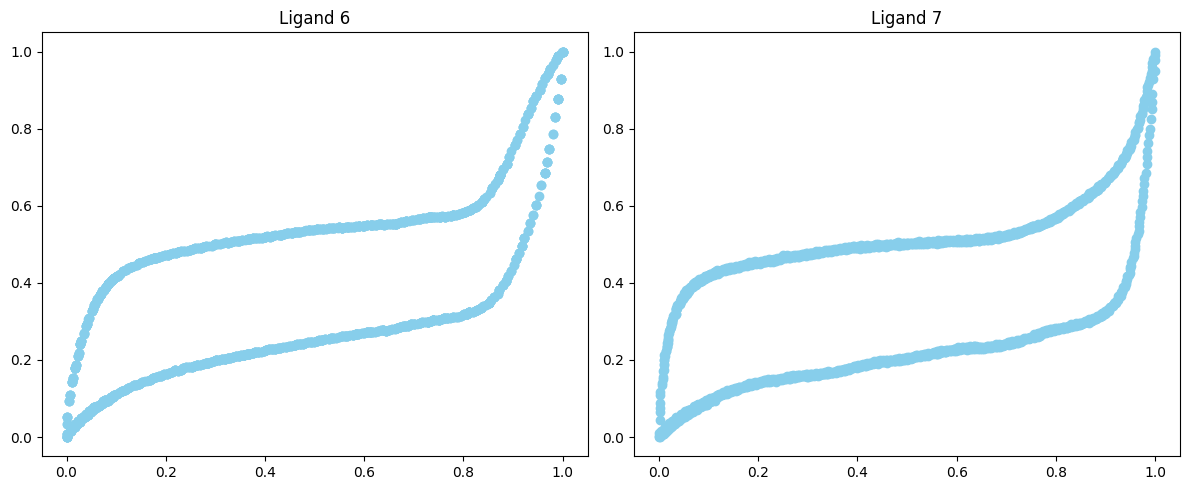
\includegraphics[width=1.0\textwidth]{figures/ligand_comparison.png}
    \caption{Ligand Six and Ligand Seven Voltammogram Comparison}
    \label{ligand_comparison}
\end{figure}
However, this misclassification is understandable. Figure \ref{ligand_comparison} shows that the voltammograms for ligand six and ligand seven are quite similar. 
\begin{figure}[h!]
  \centering
    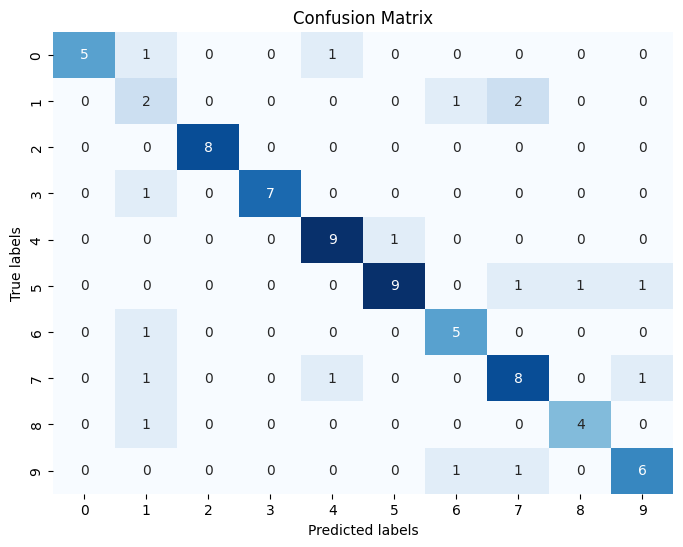
\includegraphics[width=1.0\textwidth]{figures/cv_metal_matrix.png}
    \caption{CV Metal Confusion Matrix}
    \label{cv_metal_matrix}
\end{figure}
From the confusion matrix for metals \ref{cv_metal_matrix}, metal one was difficult to recognize, with many metals being misclassified as metal one. 
\begin{figure}[h!]
  \centering
    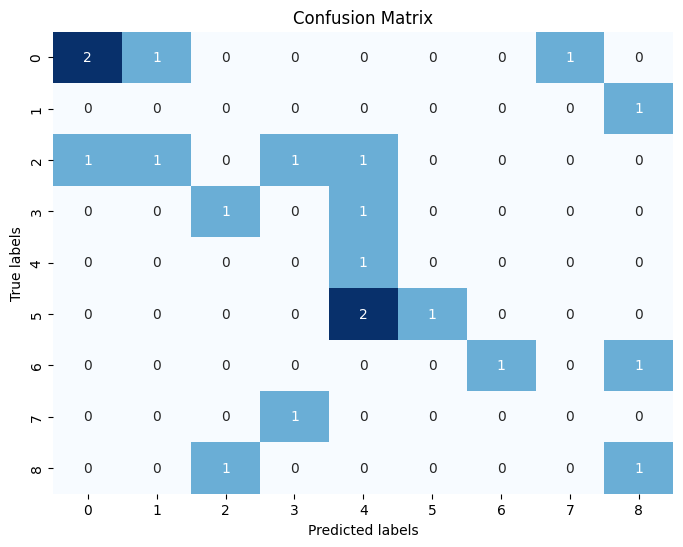
\includegraphics[width=1.0\textwidth]{figures/dpv_ligand_matrix.png}
    \caption{DPV Ligand Confusion Matrix}
    \label{dpv_ligand_matrix}
\end{figure}
\begin{figure}[h!]
  \centering
    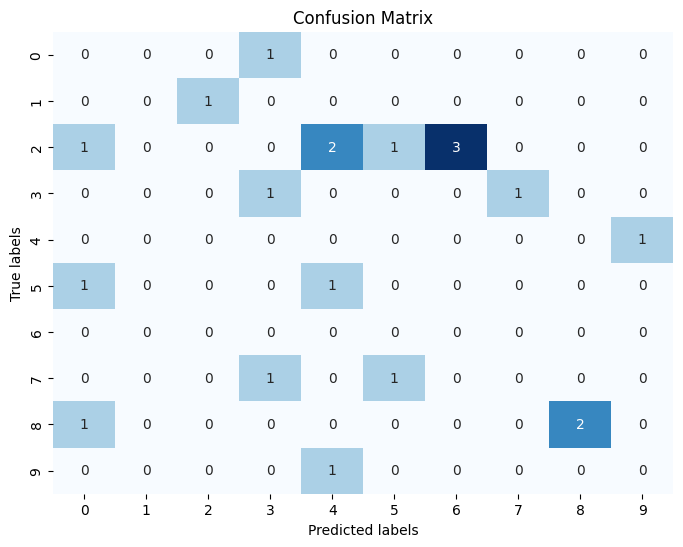
\includegraphics[width=1.0\textwidth]{figures/dpv_metal_matrix.png}
    \caption{DPV Metal Confusion Matrix}
    \label{dpv_metal_matrix}
\end{figure}
From the DPV confusion matrices seen in Figure \ref{dpv_metal_matrix} and Figure \ref{dpv_ligand_matrix}, it is hard to draw any definitive conclusions due to the dataset size. 
A major challenge in supervised learning is providing good examples during training. However, despite using a small dataset, these results are promising. This study establishes that crude CV data obtained from an economical potentiostat can be effectively encoded using CNNs. It was also shown that VAEs and CVAEs can generate high-quality, generalizable synthetic data. These findings align with recent research demonstrating that deep learning models can efficiently process CV data \cite{Hoar2022}. Although the ligand and metal labels are recorded. The results demonstrate that the encoding technique effectively captures the chemistry behind the measurements. Future research can incorporate group SELFIES within the decoder layer to predict or select from a pool of candidate redox groups identified through voltammetry or predict the compound used. 
